\chapter{Sample Software Control Algorithms}\label{flow}

\section{Temperature Control System}

\begin{figure}[htbp]
	\centering
	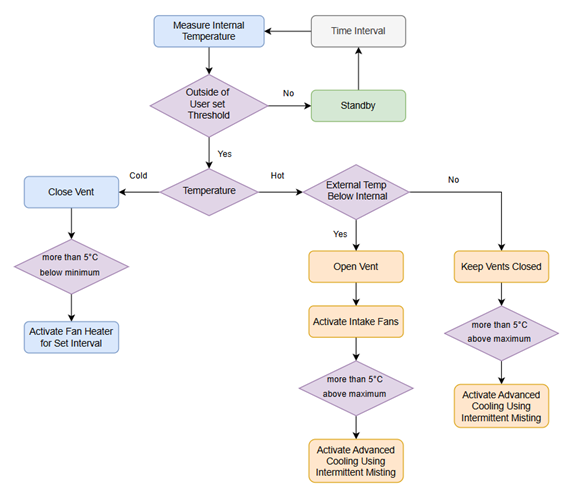
\includegraphics[width=0.75\textwidth]{figs/soft2.png}
	\caption{Temperature control}
	\label{fig:temperature_control}
\end{figure}

Temperature control is given the highest priority among all environmental parameters. The system continuously measures the internal temperature of the greenhouse and compares the readings to user-defined setpoints. When the temperature falls outside the desired range, the appropriate actuators namely the vent, fans, heater, or misters are activated or deactivated accordingly.

To prevent excessive watering, the misting system is only enabled for thermal regulation when the internal temperature exceeds the upper setpoint by at least 5 °C This is designated as 'Advanced Cooling'. This allows passive evaporative cooling to occur without over-saturating the soil. All temperature thresholds are implemented with hysteresis logic to prevent unnecessary switching and ensure stable control behavior.

\section{Airflow Control System}

\begin{figure}[H]
	\centering
	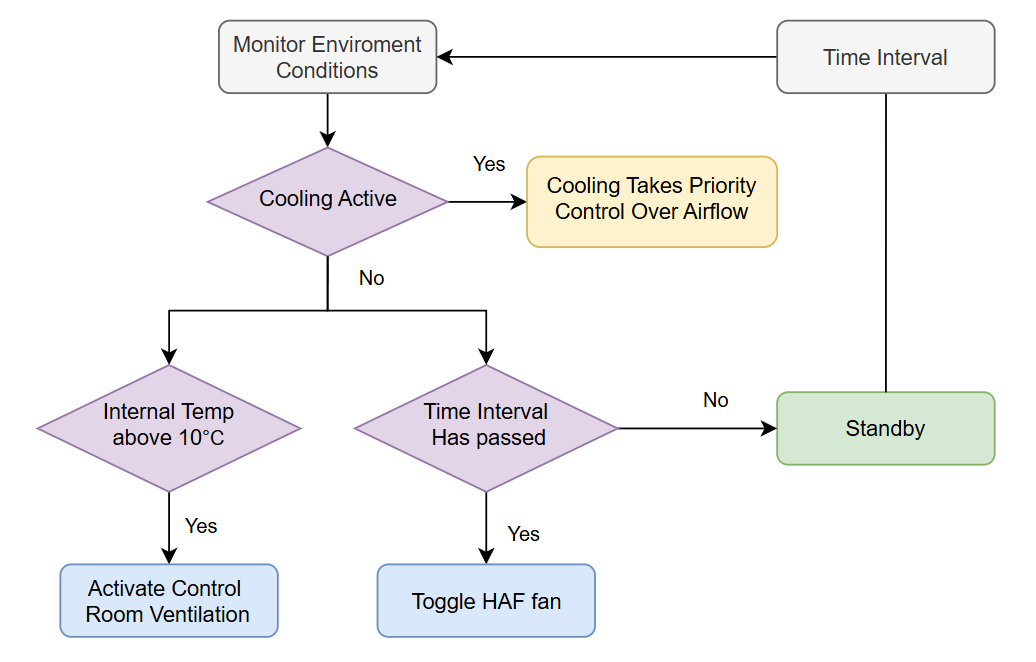
\includegraphics[width=0.6\textwidth]{figs/soft3.png}
	\caption{Airflow control}
	\label{fig:airflow_control}
\end{figure}


Airflow control is implemented according to the flowchart shown above. While temperature regulation takes priority over airflow operations, the airflow subsystem functions independently when cooling is not required. In such cases, the internal circulation fan is activated whenever the ambient temperature inside the greenhouse exceeds 10 °C, ensuring adequate ventilation and preventing electrical components from overheating. When temperature control is inactive, the external HAF/intake fan operates intermittently to maintain proper air circulation and fulfill high-airflow (HAF) requirements within the greenhouse.

\section{Irrigation Control System}
 
\begin{figure}[htbp]
	\centering
	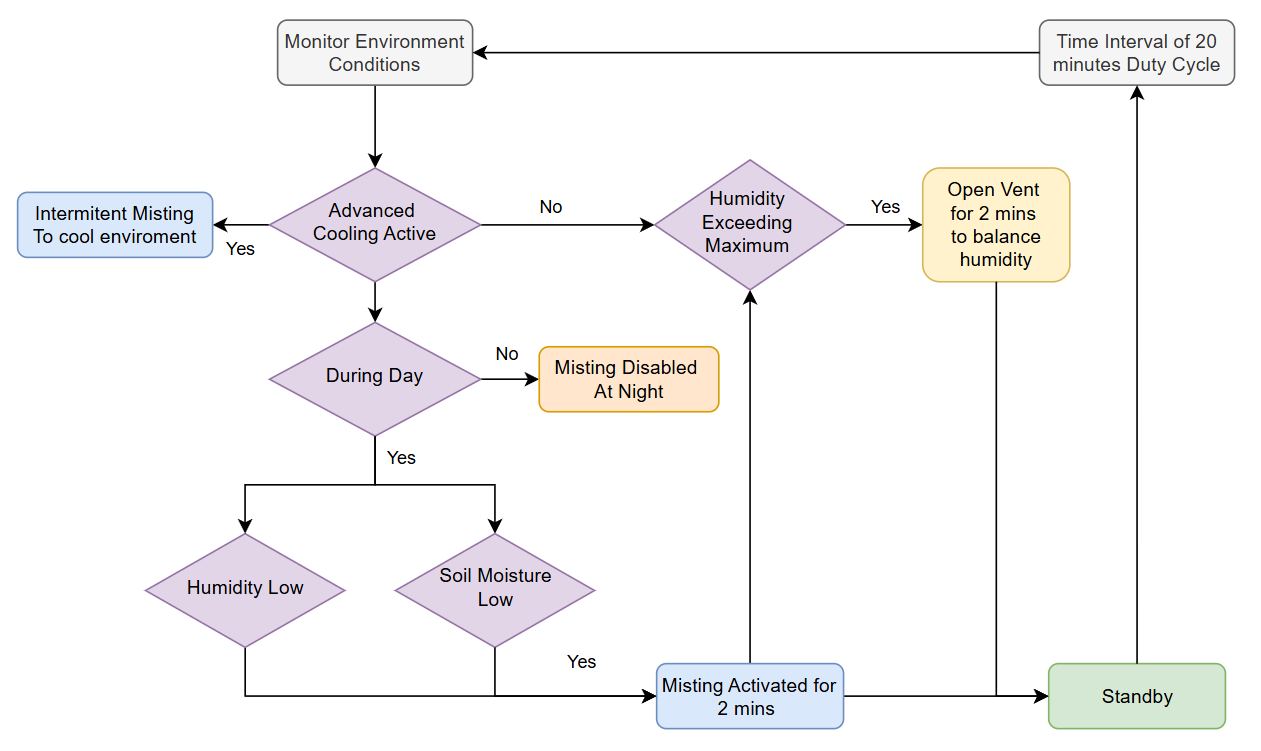
\includegraphics[width=0.8\textwidth]{figs/soft4.png}
	\caption{Irrigation control}
	\label{fig:irrigation_control}
\end{figure}

The irrigation control flowchart outlines the misting logic implemented in the system. The controller first determines whether advanced cooling is required, in such cases temperature control takes priority, and the misters are activated intermittently to promote passive evaporative cooling of the environment. When advanced cooling is not active, the system compares humidity and soil moisture levels against their respective setpoints. If either parameter falls below the desired range, misting is initiated. Misting is disabled during nighttime hours to maintain lower humidity levels, reducing the risk of fungal growth, and to prevent unwanted cooling effects that could lower temperatures below optimal levels. Hysteresis control is implemented in all misting decisions to prevent rapid cycling and ensure stable operation.

All misting operations are regulated by an overall duty cycle, allowing the misters to run for two minutes followed by a twenty-minute pause. This prevents overwatering and ensures sufficient time for sensor feedback to stabilize. Additionally, if humidity levels exceed the maximum threshold after misting, the ventilation system is temporarily activated to restore balanced humidity conditions within the greenhouse.

\section{Light Control System}

\begin{figure}[htbp]
	\centering
	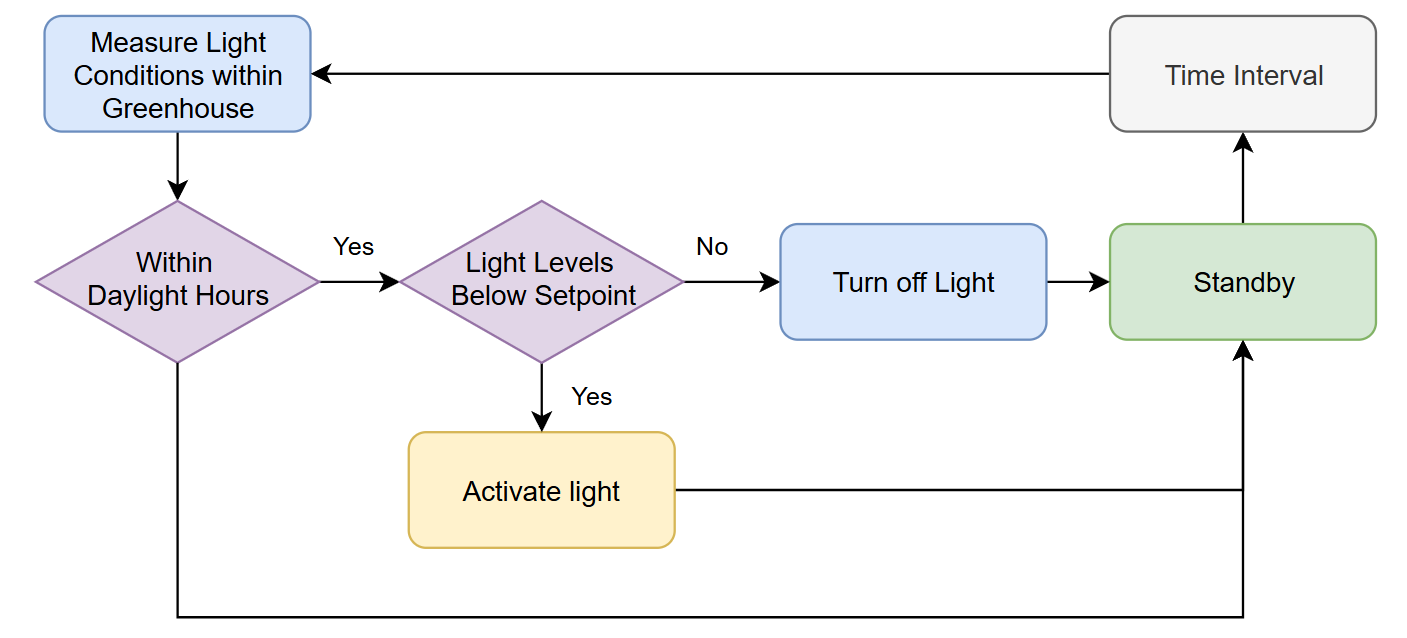
\includegraphics[width=0.6\textwidth]{figs/soft5.png}
	\caption{Light control}
	\label{fig:light_control}
\end{figure}

The light control flowchart outlines the logic governing supplemental lighting within the system. Supplemental lighting is restricted to operate only during daylight hours. When the measured light intensity falls below the desired setpoint of 200~\si{\micro\mole\per\metre\squared\per\second}, the system activates the grow lights to maintain adequate illumination for plant growth. Hysteresis logic is incorporated to prevent unnecessary on--off cycling, ensuring stable operation and reducing wear on the lighting components.
 